\chapter{Исследовательская часть}

В данном разделе будут приведены примеры работы программ,
постановка эксперимента и сравнительный анализ алгоритмов на основе
полученных данных.

\section{Технические характеристики}

Технические характеристики устройства, на котором выполнялось тестирование,
следующие.

\begin{itemize}
	\item Операционная система: macOs Monterey 12.4\cite{ubuntu}.
	\item Память: 16 GiB.
	\item Процессор: 2,6 GHz 6‑ядерный процессор Intel Core i7\cite{intel}.
\end{itemize}

Тестирование проводилось на ноутбуке, включенном в сеть электропитания.
Во время тестирования ноутбук был нагружен только встроенными приложениями
окружения, а также непосредственно системой тестирования.

\section{Время выполнения алгоритмов}

Результаты замеров приведены в таблицах \ref{tbl:best}, \ref{tbl:wor} и \ref{tbl:random}.

На рисунках \ref{img:1}, \ref{img:2} и \ref{img:3}, приведены графики
зависимостей времени работы алгоритмов сортировки от размеров массивов
на отсортированных, обратно отсортированных и случайных данных.

\begin{table}[h]
	\begin{center}
		\caption{Время работы алгоритмов сортировки на отсортированных данных (мкс)}
		\label{tbl:best}
		\begin{tabular}{|c|c|c|c|}
			\hline
			Размер & Бин. деревом &  Побитовая &  Бусинами \\
			\hline
			1 & 4 & 69 & 3\\
			\hline
			1000 & 22511 & 526 & 107172\\
			\hline
			2000 & 108509 & 1110 & 549337\\
			\hline
			3000 & 206095 & 955 & 1020739\\
			\hline
			4000 & 358984 & 976 & 1718596\\
			\hline
			5000 & 575893 & 1288 & 2628007\\
			\hline
			6000 & 773042 & 1274 & 3468504\\
			\hline
			7000 & 1169221 & 1404 & 5109550\\
			\hline
			8000 & 1395231 & 1731 & 6529044\\
			\hline
			9000 & 1648723 & 2126 & 8070125\\
			\hline
			10000 & 2052951 & 2011 & 10733265\\
			\hline
		\end{tabular}
	\end{center}
	
\end{table}

\begin{table}[h]
	\begin{center}
		\caption{ Время работы алгоритмов сортировки на обратно	отсортированных данных (мкс)}
		\label{tbl:wor}
		\begin{tabular}{|c|c|c|c|}
			\hline
			Размер & Бин. деревом &  Побитовая &  Бусинами \\
			\hline
			1 & 2 & 67 & 4\\
			\hline
			1000 & 23829 & 376 & 104320\\
			\hline
			2000 & 89826 & 627 & 449222\\
			\hline
			3000 & 198398 & 987 & 958754\\
			\hline
			4000 & 356747 & 1148 & 1724451\\
			\hline
			5000 & 518240 & 1221 & 2427763\\
			\hline
			6000 & 815127 & 1289 & 3550234\\
			\hline
			7000 & 1046235 & 1482 & 4790517\\
			\hline
			8000 & 1373987 & 1558 & 6534334\\
			\hline
			9000 & 1629427 & 1736 & 8008745\\
			\hline
			10000 & 2103647 & 1981 & 9988846\\
			\hline
		\end{tabular}
	\end{center}
	
\end{table}

\begin{table}[h]
	\begin{center}
		\caption{ Время работы алгоритмов сортировки на случайных данных (мкс)}
		\label{tbl:random}
		\begin{tabular}{|c|c|c|c|}
			\hline
			1 & 2 & 67 & 4\\
			\hline
			1000 & 23829 & 376 & 104320\\
			\hline
			2000 & 89826 & 627 & 449222\\
			\hline
			3000 & 198398 & 987 & 958754\\
			\hline
			4000 & 356747 & 1148 & 1724451\\
			\hline
			5000 & 518240 & 1221 & 2427763\\
			\hline
			6000 & 815127 & 1289 & 3550234\\
			\hline
			7000 & 1046235 & 1482 & 4790517\\
			\hline
			8000 & 1373987 & 1558 & 6534334\\
			\hline
			9000 & 1629427 & 1736 & 8008745\\
			\hline
			10000 & 2103647 & 1981 & 9988846\\
			\hline
		\end{tabular}
	\end{center}
	
\end{table}
\clearpage

\begin{figure}[h!]
\centering
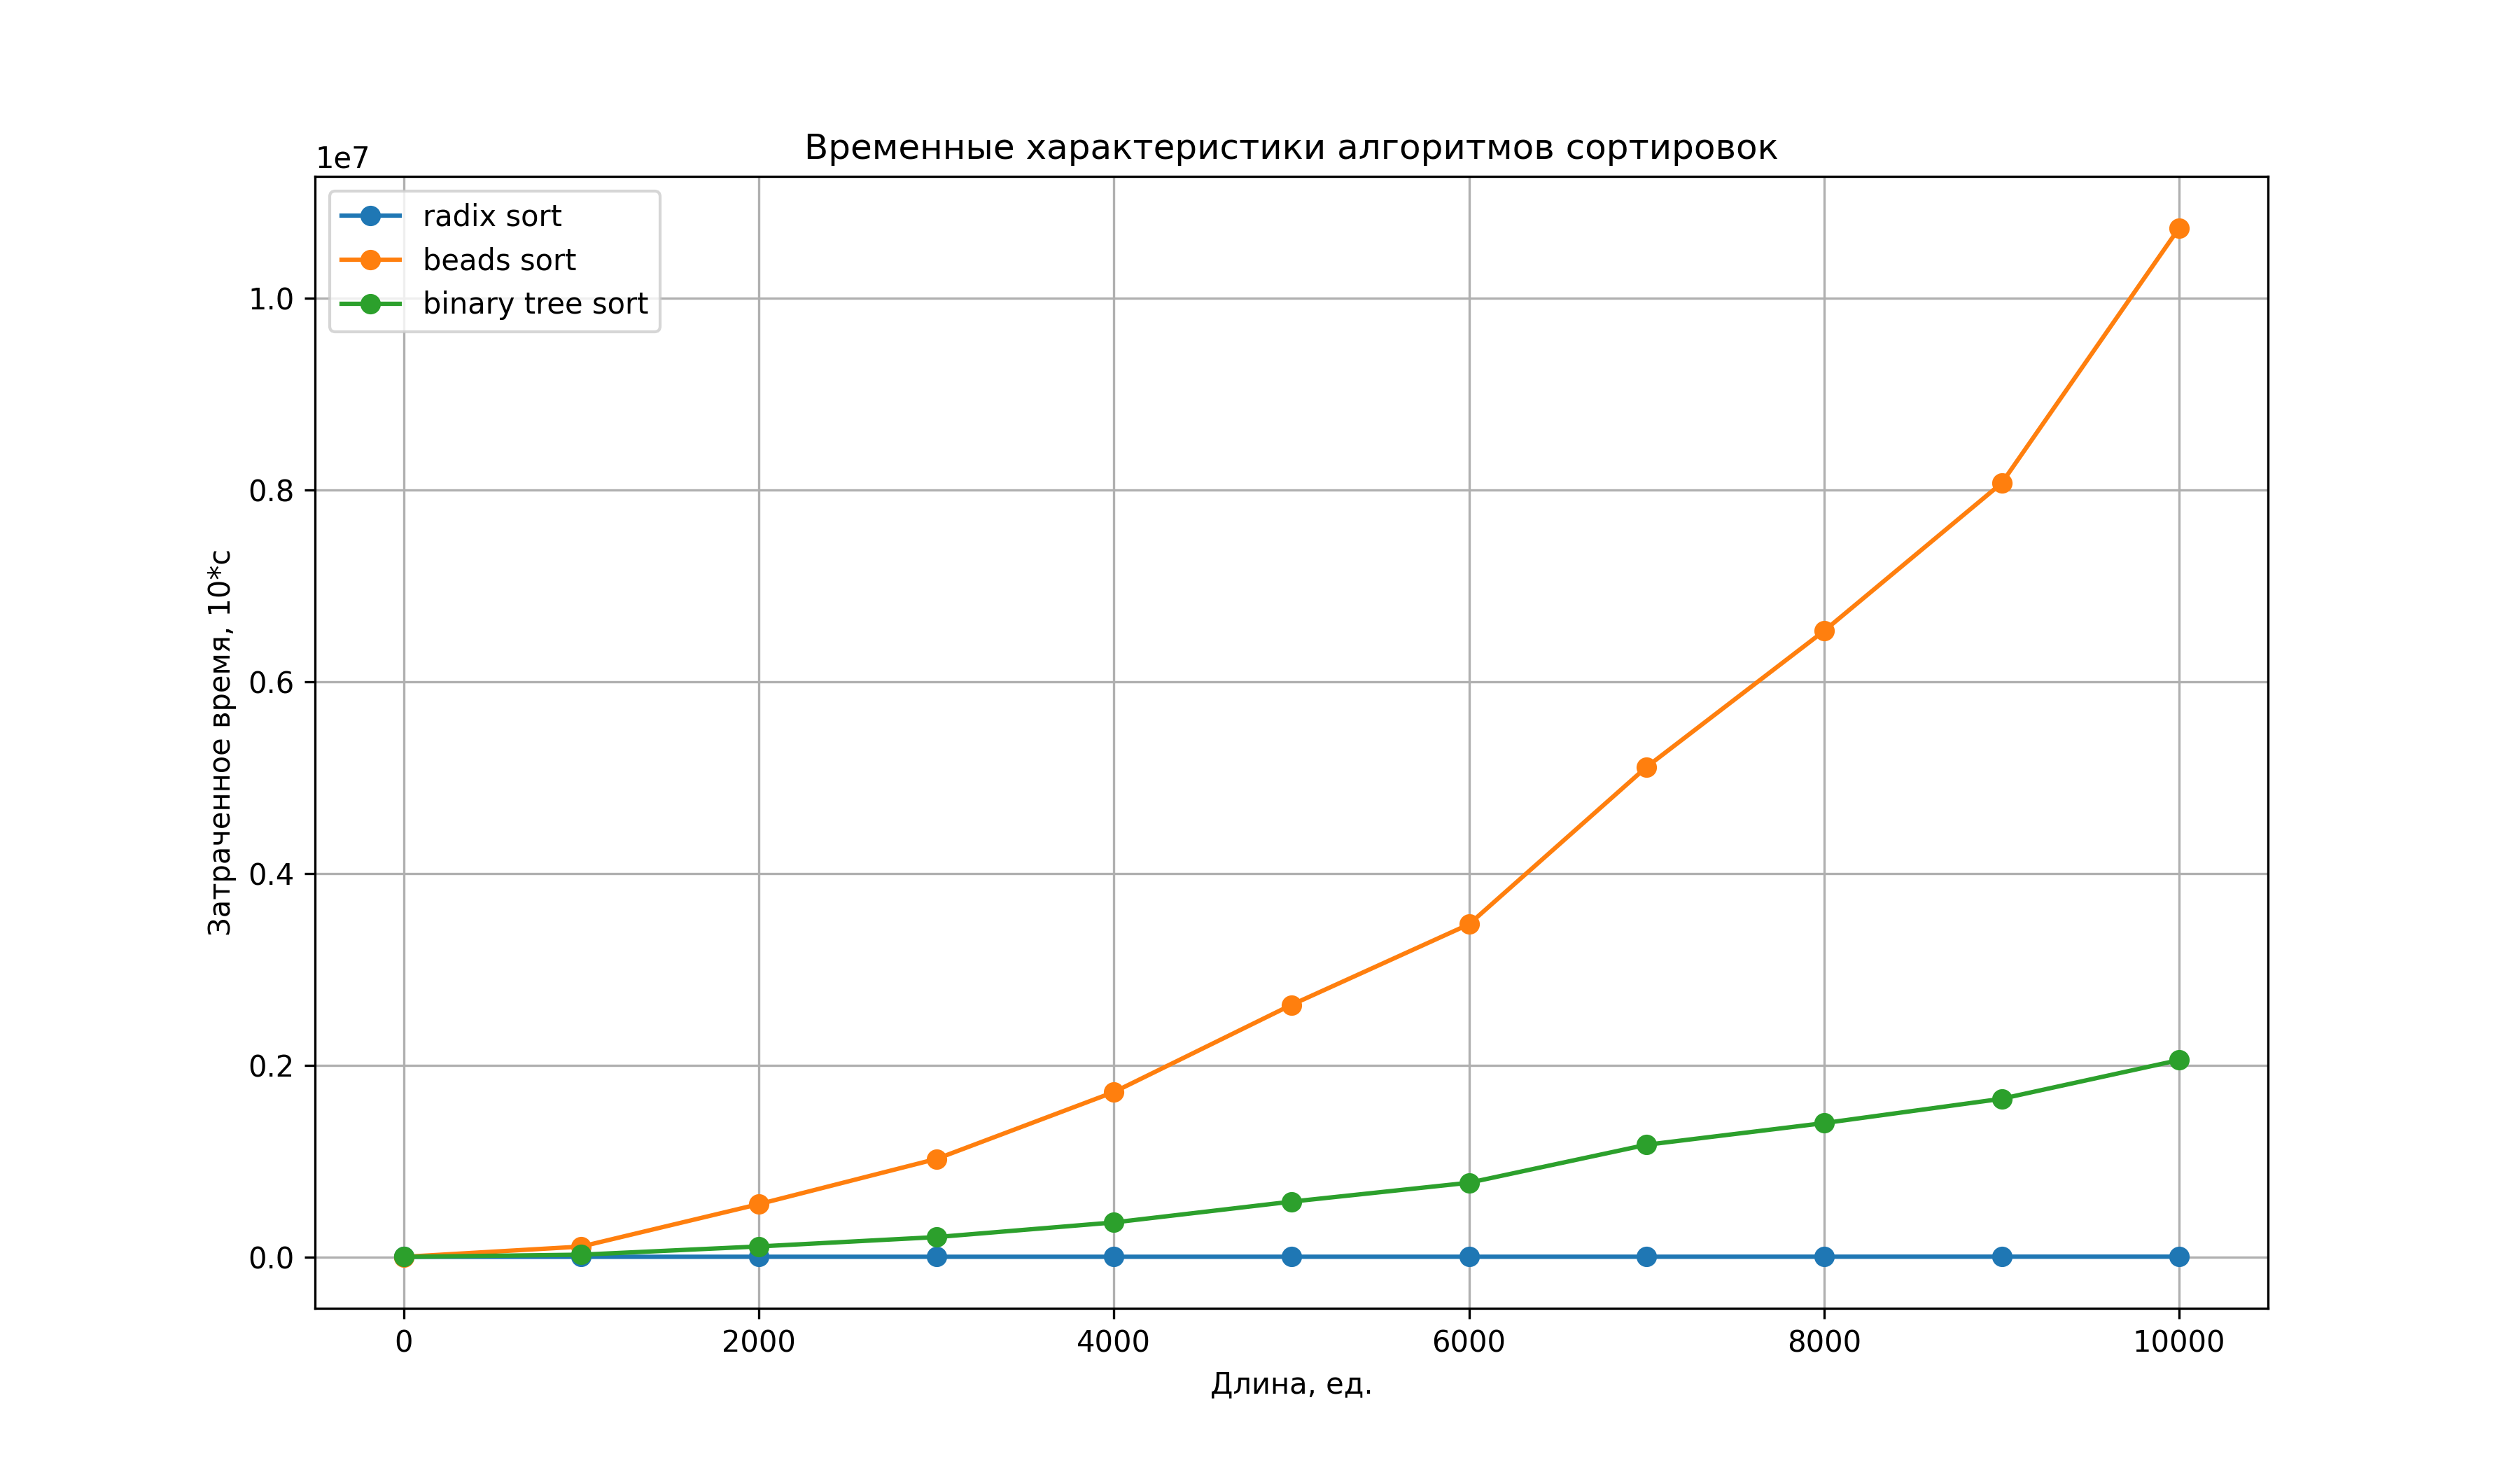
\includegraphics[width=1\linewidth]{inc/img/sort_time_graph_0.png}
\caption{График зависимости времени сортировки от количества элементов в коллекции на отсортированных данных}
\label{gra:sor}
\end{figure}

\begin{figure}[h!]
\centering
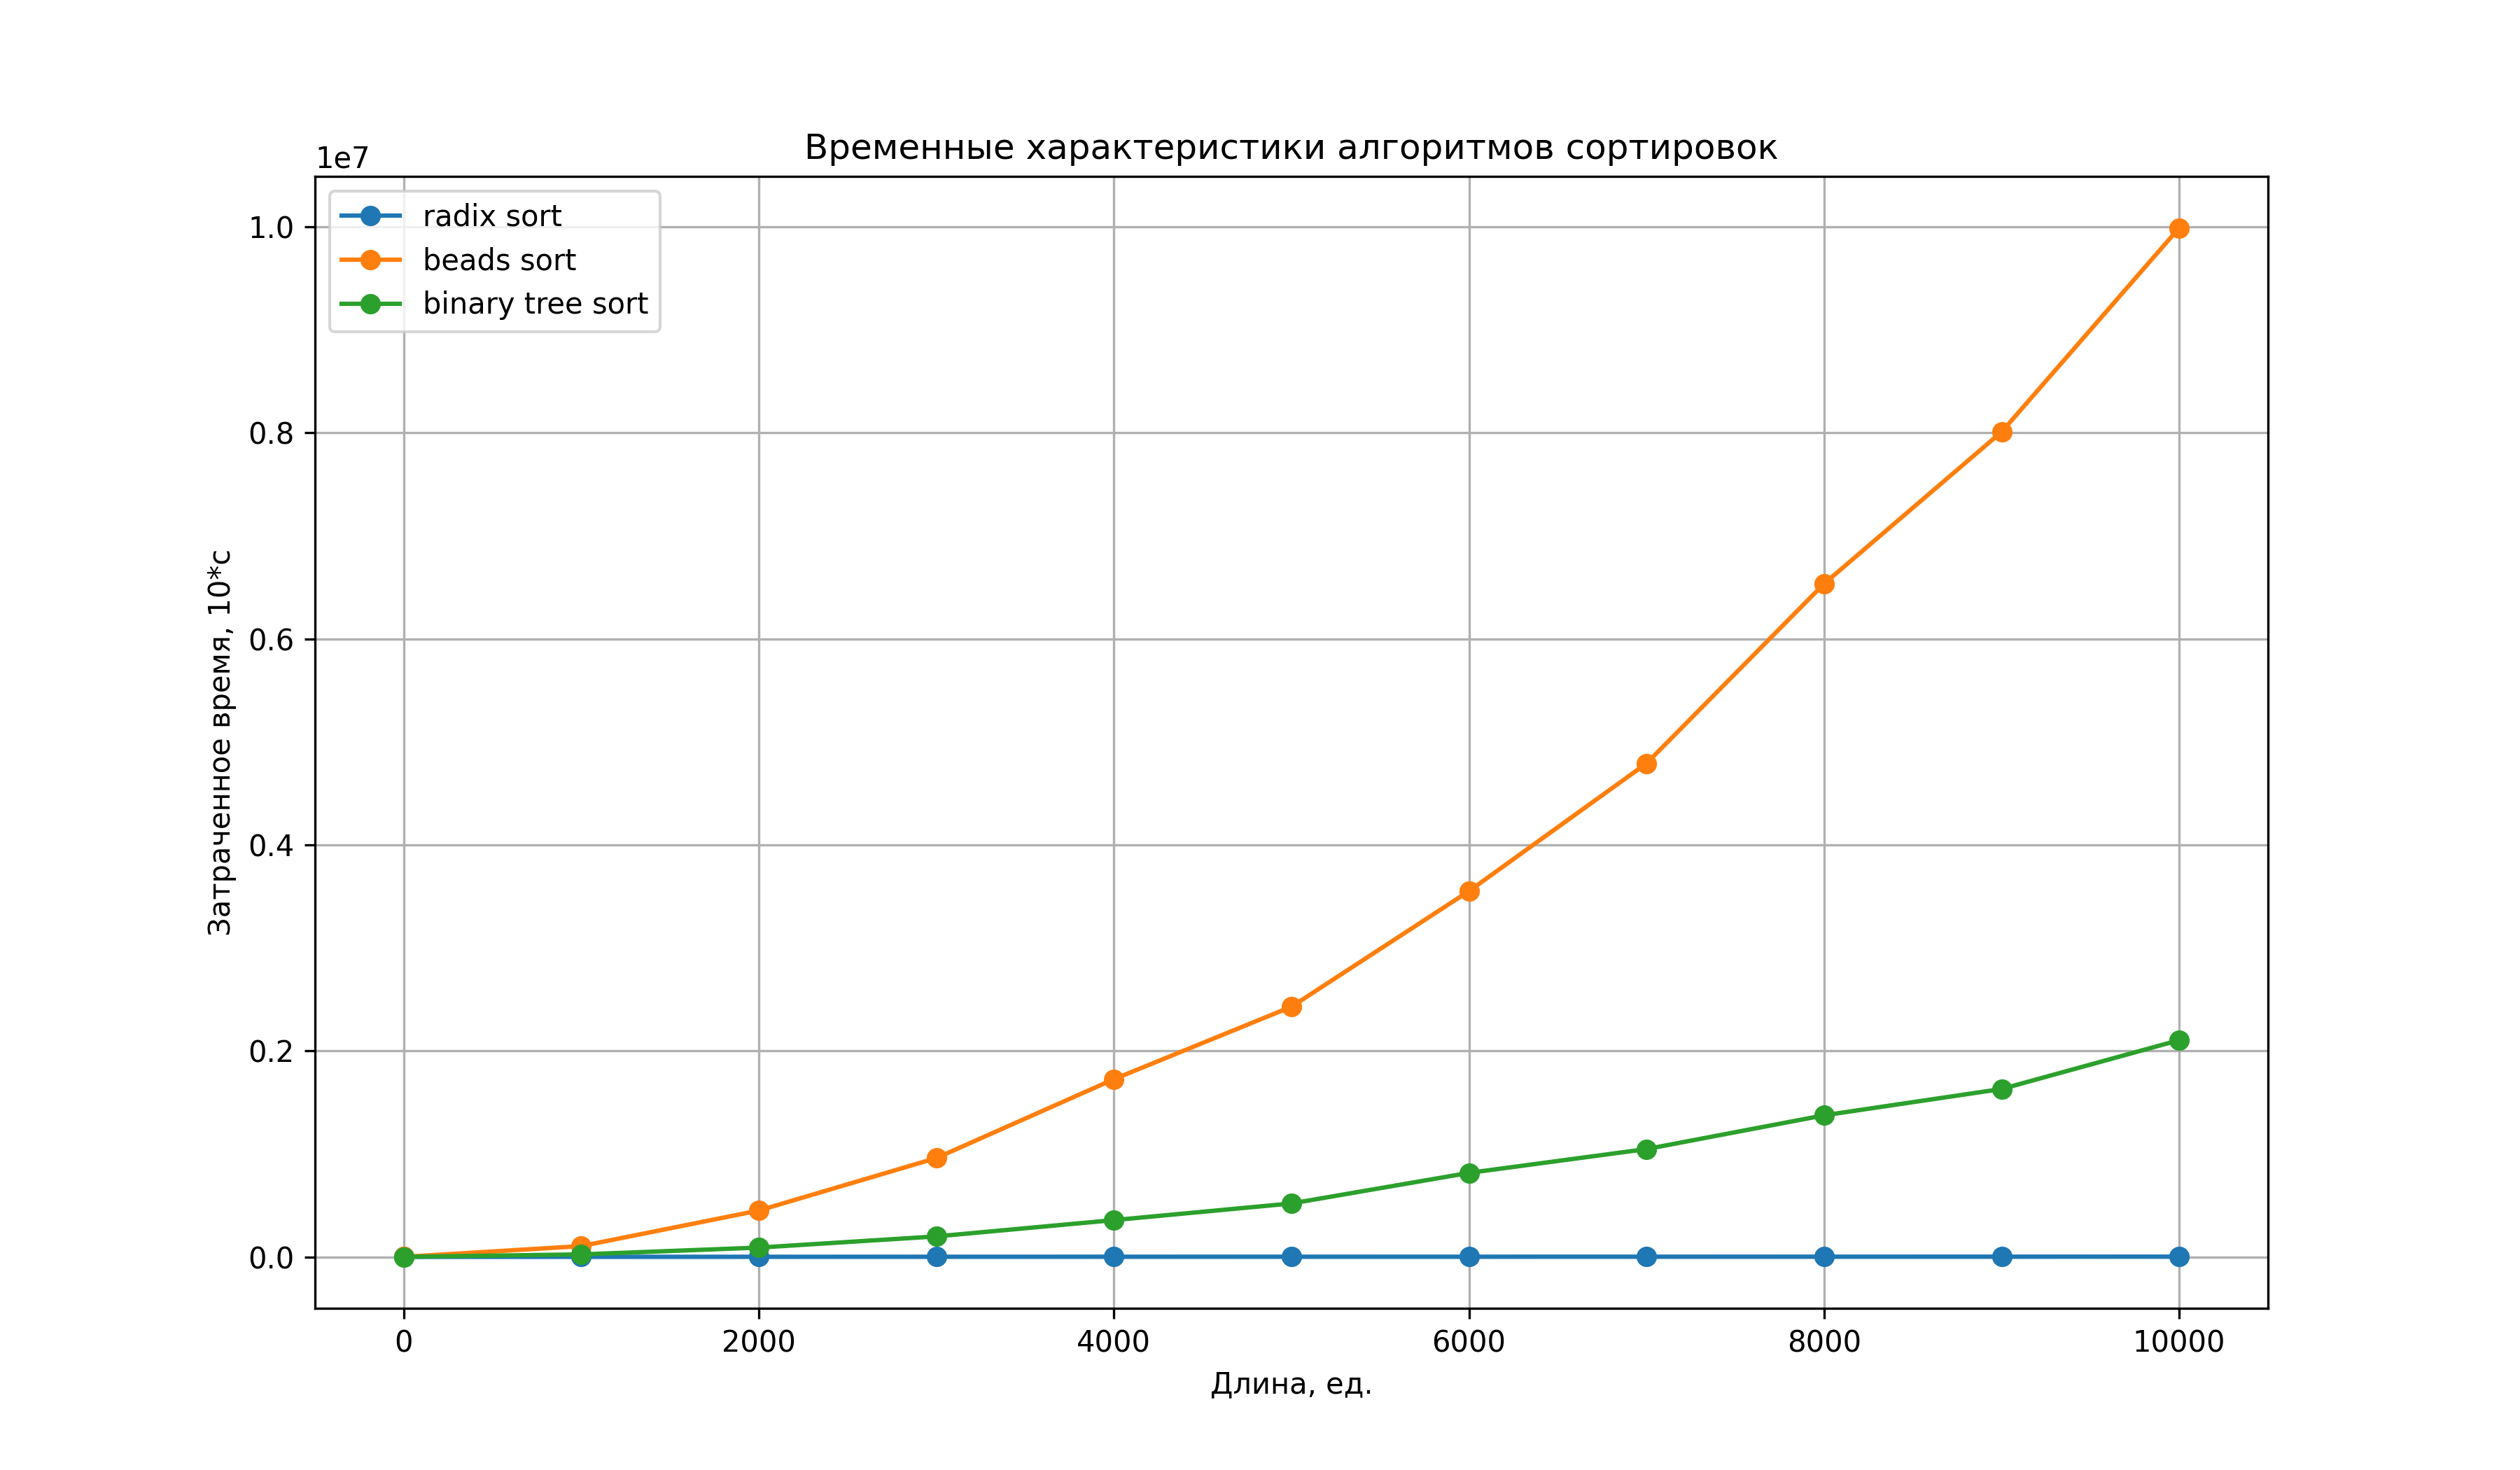
\includegraphics[width=1\linewidth]{inc/img/sort_time_graph_1.png}
\caption{График зависимости времени сортировки от количества элементов в коллекции на данных, отсортированных в обратном порядке}
\label{gra:rsor}
\end{figure}

\begin{figure}[h!]
\centering
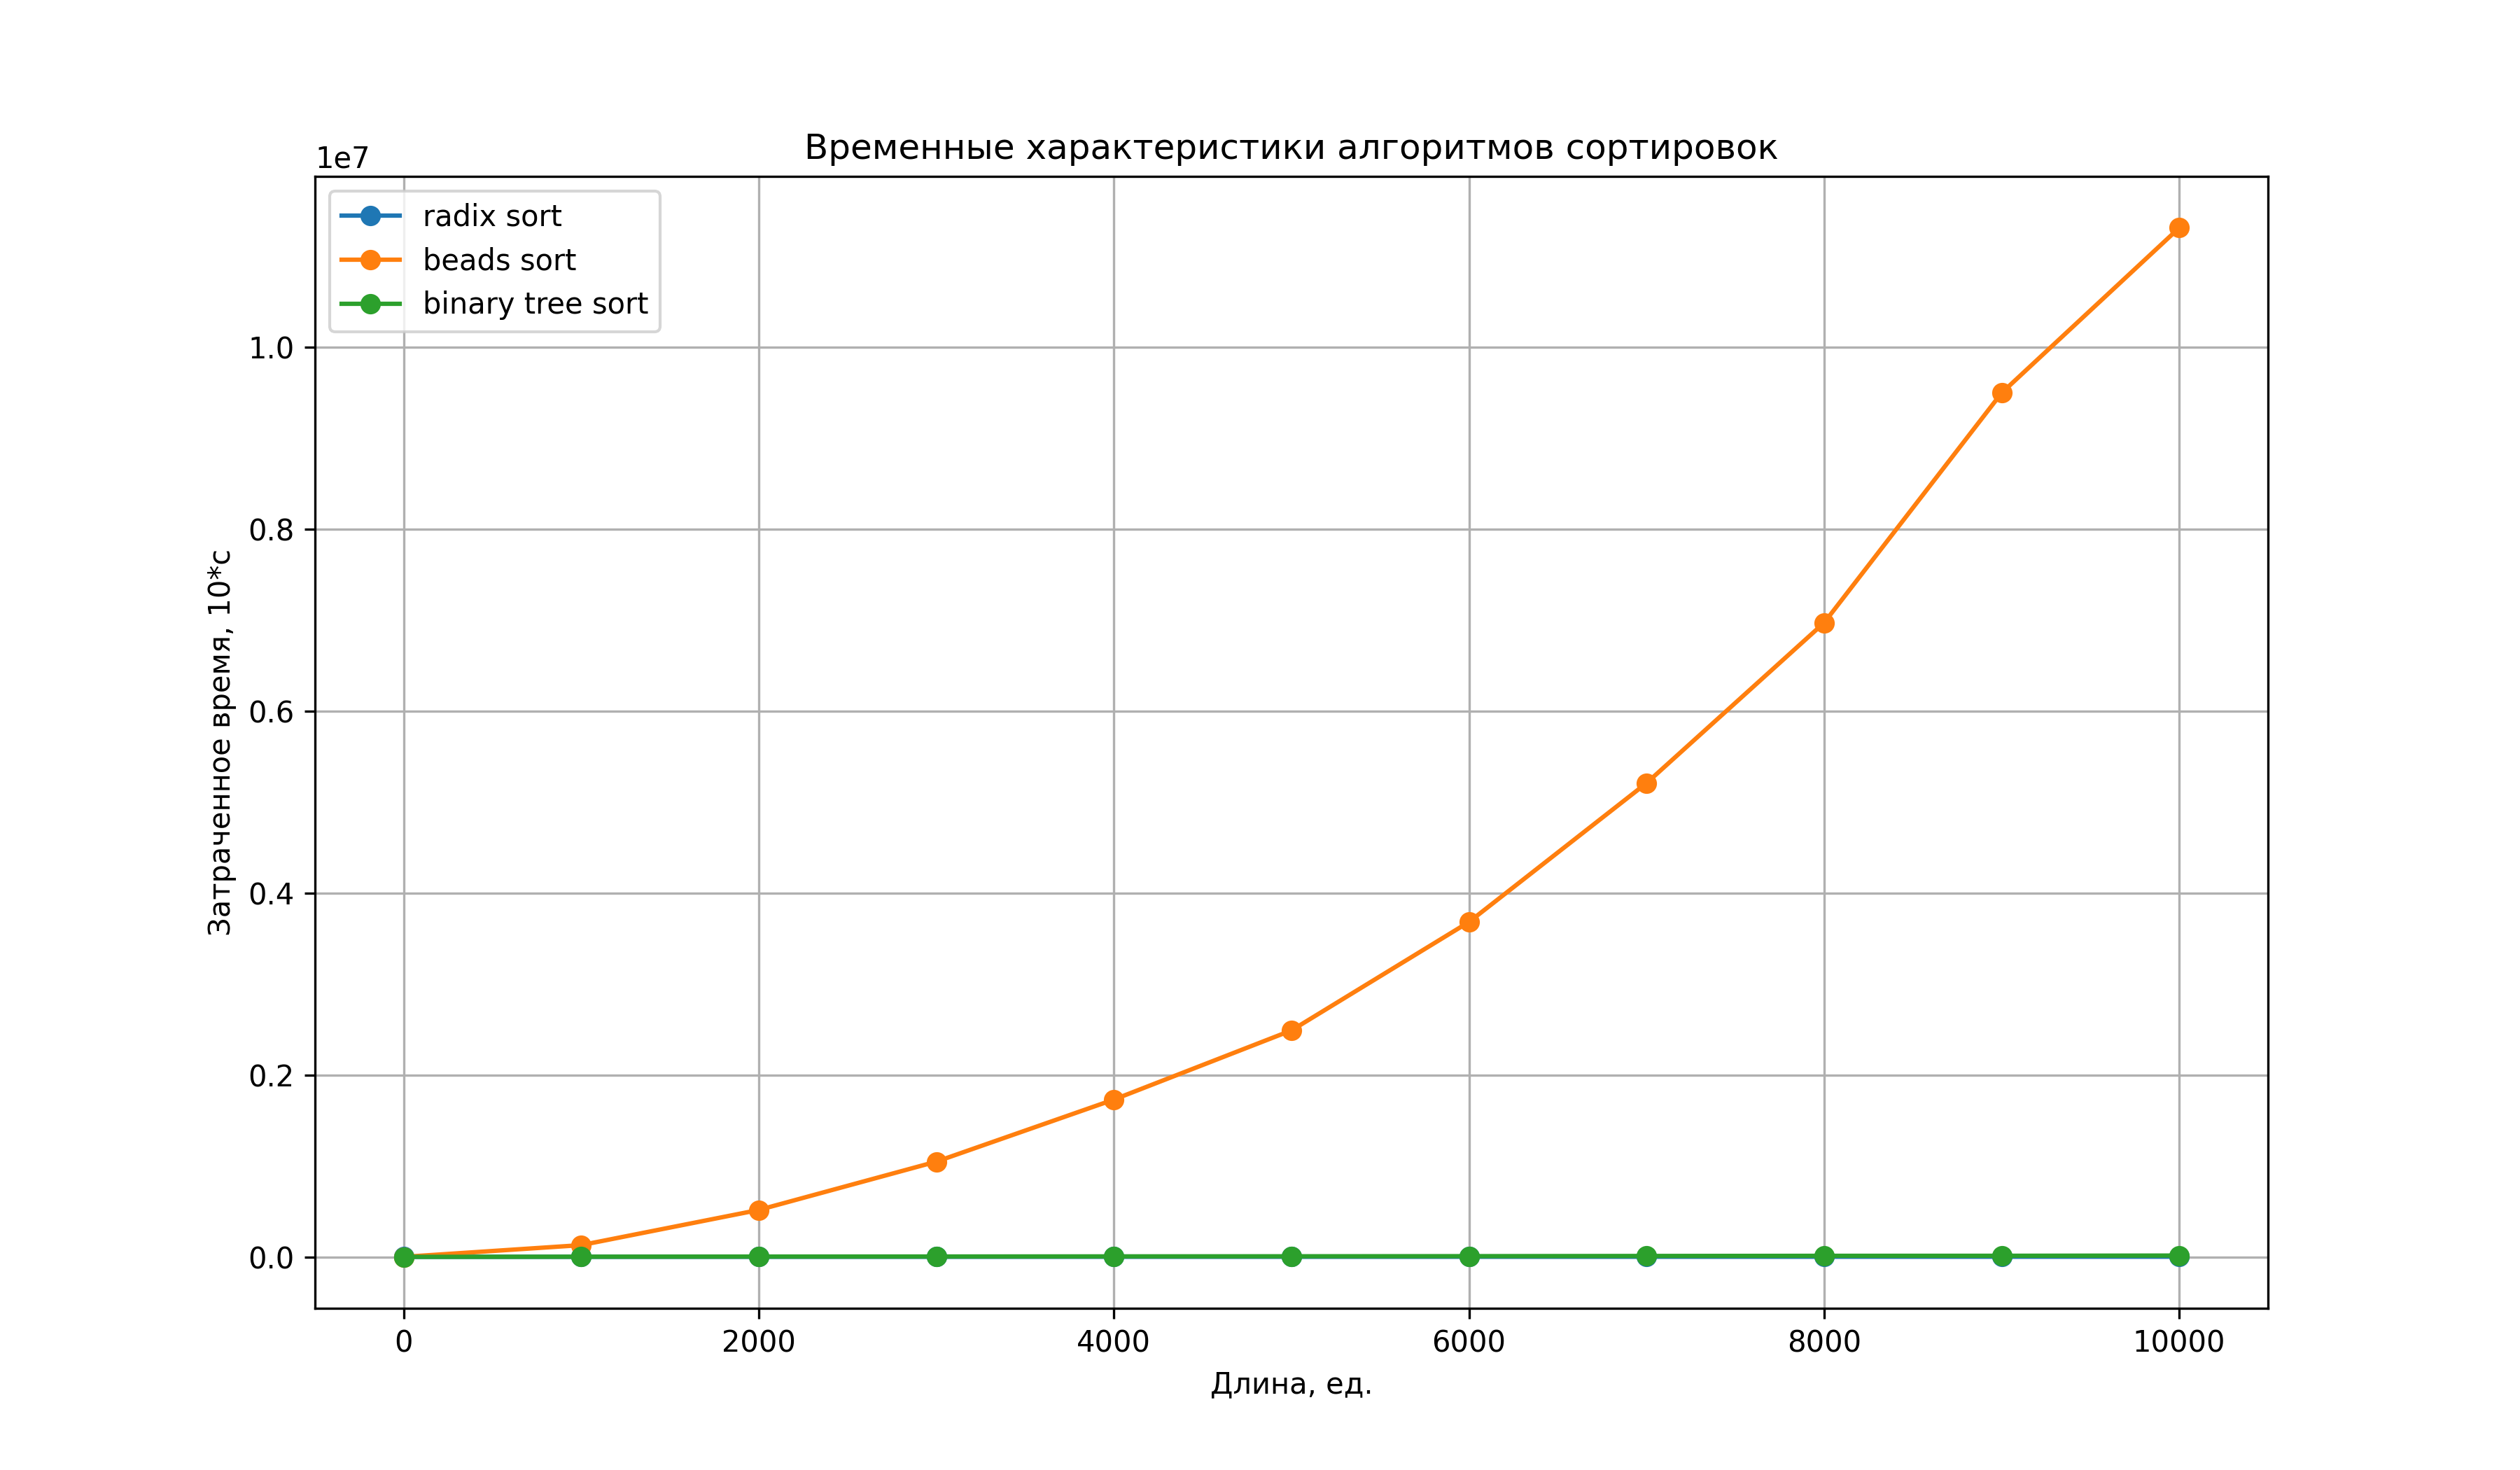
\includegraphics[width=1\linewidth]{inc/img/sort_time_graph_2.png}
\caption{График зависимости времени сортировки от количества элементов в коллекции на данных, сформированных случайным образом}
\label{gra:rand}
\end{figure}

\section*{Вывод}

Алгоритм сортировки бусинами является крайне неэффективным и может представлять интерес лишь в учебных целях.

Алгоритм сортировки бинарным деревом (при использовании обычного ДДП) деградирует до сложности $O(n^2)$ на отсортированных данных. Из этого можно сделать вывод, что при наличии  вероятности появления отсортированных (или близких к таковым) входных данных лучше использовать какой-либо вид сбалансированных деревьев. Таковыми могут быть АВЛ, красно-черное дерево и некоторые другие.

Алгоритм побитовой сортировки является  эффективным способом сортироки данных, каждый элемент которых, имеет небольшой размер.


